\documentclass[11pt]{article}
\usepackage[margin=3cm]{geometry}
\usepackage[swedish]{babel}
\usepackage[utf8]{inputenc}
\usepackage[T1]{fontenc}
\usepackage{fancyhdr}
\usepackage{ragged2e}
\usepackage{titling}
\usepackage{graphicx}
\usepackage{pbox}
\usepackage{tabularx}
\usepackage{longtable}
\usepackage{tabu}
\usepackage{url}
\usepackage{float}
\usepackage{verbatim}

\begin{comment}
Lägg till vinkelaccele
\end{comment}


\graphicspath{ {../images/} }
\newcommand{\subtitle}[1]{%
  \posttitle{%
    \par\end{center}
    \begin{center}\large#1\end{center}
    \vskip0.5em}%
}

\pagestyle{fancy}


\date{}
\pagenumbering{roman}
\chead{Undsättningsrobot}
\rhead{2015-01-29}
\lhead{}
\lfoot{
	TSEA56 
	\\
	Systemskiss
}
\rfoot{
	Projektgrupp 2
	\\
	e-post: adnbe196@student.liu.se
}

\begin{document}
\begin{titlepage}
\begin{center}
{\Large\bfseries TSEA56 - Kandidatprojekt i elektronik \\ Systemskiss}\\
%
\vspace{2\baselineskip}
%
Version 0.1\\
\vspace{2\baselineskip}
%
Grupp 2 \\
Agafonov, Nikolaj, 
\texttt{nikag669}
\\
Berberovic, Adnan, 
\texttt{adnbe196}
\\
Brorsson, Andreas, 
\texttt{andbr981}
\\
Fridborn, Fredrik, 
\texttt{frefr166}
\\
Oprea, Robert, 
\texttt{robop806}
\\
Skytt, Måns, 
\texttt{mansk700}

\vspace{2\baselineskip}
2015-02-13

\vspace{25\baselineskip}
Status
\begin{longtable}{|l|l|l|} \hline

Granskad &
 Robert Oprea &
 2015-02-16 \\ \hline
Godkänd &
 &
 \\ \hline
 
\end{longtable}

\end{center}
\end{titlepage}

\pagebreak
\begin{center}

\section*{PROJEKTIDENTITET}
2015/VT, Undsättningsrobot Gr. 2
\\
Linköpings tekniska högskola, ISY
\\[0.5in]
\begin{table}[h]
\begin{tabular}{|l|p{0.3\linewidth}|l|l|} \hline
Namn & Ansvar & Telefon & E-post \\[0.1in] \hline
Nikolaj Agafonov & Dokumentansvarig (DA) & 072-276 99 46 & nikag669@student.liu.se \\ \hline
Adnan Berberovic & Projektledare (PL) & 070-491 96 07 & adnbe196@student.liu.se \\ \hline
Andreas Brorsson & Testansvarig (TA) & 073-524 44 60 & andbr981@student.liu.se \\ \hline
Fredrik Fridborn & Designansvarig Sensormodul (DSE) & 073-585 52 01 & frefr166@student.liu.se \\ \hline
Robert Oprea & Designansvarig Styrmodul (DST) & 070-022 10 18 & robop806@student.liu.se \\ \hline
Måns Skytt & Designansvarig Kommunikationsenhet (DK) & 070-354 28 84 & mansk700@student.liu.se \\ \hline
\end{tabular}
\end{table}

E-postlista för hela gruppen: adnbe196@student.liu.se
\\[1in]
Kund: Kent Palmkvist, 581 83 Linköping,
Kundtelefon: 013-28 13 47, kentp@isy.liu.se
\\[1in]
Kursansvarig: Tomas Svensson, 013-28 13 68, tomass@isy.liu.se
\\
Handledare: Kent Palmkvist, 013-28 13 47, kentp@isy.liu.se
\end{center}
\pagebreak

\tableofcontents

\pagebreak

\section*{Dokumenthistorik}
\begin{table}[h]
\begin{tabular}{|l|l|l|l|l|} \hline

Version & 
Datum & 
Utförda förändringar & 
Utförda av & 
Granskad \\[0.1in] \hline
0.1 &
2015-02-13 & 
Första utkastet & 
Grupp 2 & 
Robert Oprea \\ \hline

0.2 &
2015-02-18 & 
Andra utkastet & 
Måns Skytt& 
 \\ \hline

\end{tabular}
\end{table}


\pagebreak

\pagenumbering{arabic}

\begin{flushleft}

\section{Inledning}
Denna projektskiss är en del av förarbetet till kandidatprojektet i Elektronik (TSEA56) och detta är en översiktlig beskrivning av hela systemet samt dess ingående delsystem. Projektet utförs på uppdrag av en beställare. 

\subsection{Syfte och mål}
Syftet med projektet är att tillverka en undsättningsrobot som ska tjäna som prototyp för att testa de olika ingående delsystemens funktionalitet samt den autonoma styrningen. 

Målet med projektet är att tillhandahålla en så väl fungerande prototyp av en autonom undsättningsrobot som möjligt, inom ramarna för projektet.


\subsection{Användning}
Roboten är tänkt att användas i ett grottsystem (läs spelregler) för att hitta och undsätta personer som fastnat. Roboten ska arbeta autonomt för att hitta kortaste vägen till de nödställda för att sedan leverera nödmaterial så fort som möjligt. Roboten ska även gå att styra från en dator med enkla kommandon tex styra fram, bakåt, svänga och rotera.


\subsection{Definitioner}
Eventuella definitioner

\section{Systemöversikt}
Systemet kan ses i sin tänkta miljö i Figur  \ref{figure:Systemöversikt}.
Roboten kommunicerar med en PC via blåtandslänk. Positionsdata skickas kontinuerligt från roboten, som styrs autonomt, till PC:n där användaren kan utläsa värden.

\begin{figure}[H]
\centering
\includegraphics[width=0.8\textwidth]{system_omgivning}
\caption{Systemet i sin tänkta miljö}
\label{figure:Systemöversikt}
\end{figure}

\subsection{Grov beskrivning av systemet}
Sensorerna på roboten läser av avstånden till närliggande väggar för att hitta vägar att åka vidare på. Sensorerna kollar även så att det inte ligger hinder i vägen. Med hjälp av sensorernas data kommer roboten bygga upp en karta om vart den är, vart väggar finns och vart den redan har varit. Med hjälp av kartan ska roboten själv kunna ta beslut om vart den ska åka vidare med hjälp av styrmodulen.
Styrmodulen har inbyggd reglering för att åka centrerat i grottan och ta svängar utan att fastna. När roboten har hittat fram till de nödställda ska den själv kunna läsa av kartan och ta kortase vägen tillbaka för att plocka upp last som den sedan ska kunna köra kortaste vägen fram till den nödställde igen. Under tiden roboten kör runt autonomt i grottan ska den skicka data via blåtand tillbaka till en dator som sedan kan presentera tex en karta, hastighet och riktning.    
 
\subsection{Ingående delsystem}
Systemet kan delas upp i 4 moduler, delsystem, som ska fungera oberoende av varandra. Dessa system/moduler består även dessa av delsystem.


\begin{table}[ht]

\centering
\begin{tabular}{c l}
Delsystem 1:&
Sensormodul \\

Delsystem 2:&
Styrmodul \\

Delsystem 3:&
Kommunikationsmodul \\

Delsystem 4:&
PC \\
\end{tabular}
\caption{Ingående moduler}
\label{tab:Moduler}
\end{table}


\bigskip

Sensormodulen består av ett antal sensorer som samlar in data om omgivningen och en mikroprocessor som processerar denna data för att sedan skicka information om omgivningen till styrmodulen. Styrmodulen består även den av en mikroprocessor som utför beräkningar och tar beslut. Motorer, gripklo och LCD-display ingår även det i vad som räknas till styrmodulen.

\begin{figure}[H]
\centering
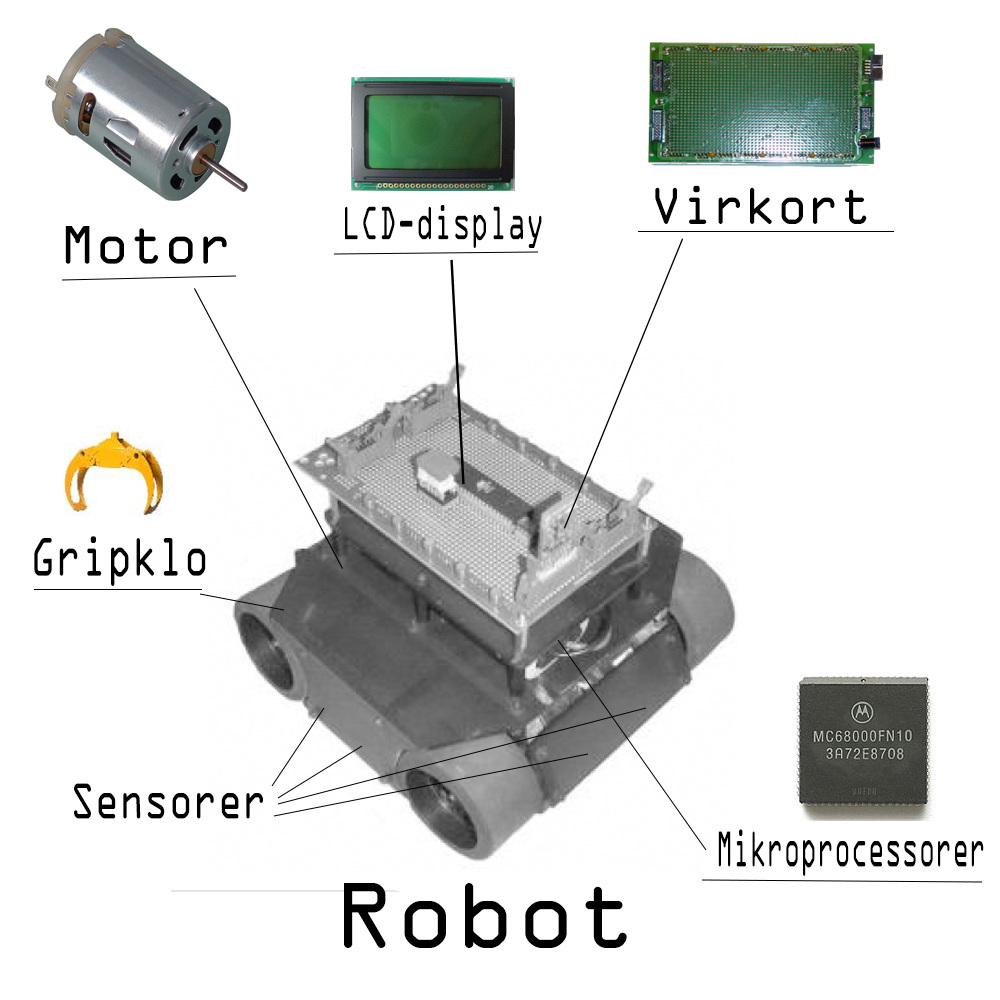
\includegraphics[width=0.3\textwidth]{Robot_moduler}
\caption{Robot med vissa delmoduler}
\label{figure:robot}
\end{figure}

Kommunikationsmodulen och PC:n består båda av bluetoothsändare och mottagare för dataöverföring. Kommunikationsmodulen har även den en mikroprocessor.

\bigskip

\begin{table}[ht]

\centering
\begin{tabular}{l l}
Sensormodul:&
Microprocessor, Sensorer \\

Styrmodul:&
Microprocessor, LCD-Display, Motorer, Gripklo\\

Kommunikationsmodul:&
Microprocessor, blutetooth- sändare/mottagare  \\

PC:&
Laptop, Bluetooth- sändare/mottagare \\
\end{tabular}
\caption{Modulers interna delsystem}
\label{tab:Delmoduler}
\end{table}

\subsection{Mikro- kontroller/processor}
Valet av mikrokontroller kommer hamna på en \textit{ATMegaXX} där typen kommer behöva specificeras när det minne och den snabbhet som krävs specificerats mer.


\subsection{Intermodulär kommunikation}
Den intermodulära kommunikationen kommer ske seriellt med ett av följande två gränssnitt: I2C eller SPI. Mest troligt I2C på grund av flera faktorer, bland annat på grund av den i teorin stödjer flera "masters" (mikrokontroller). Om I2C används kommer alla moduler ha gemensam I2C-buss. \\
\bigskip
Som kan ses i Figur \ref{fig:Intermodulär_Komm} är planen att kommunikationen mellan sensor- och styrmodul ska vara enkelvägs. Detta kan dock komma att ändras, men i nuläget krävs endast enkelvägskommunikation. Mellan styr- och kommunikationsmodulen krävs dock dubbelvägskommunikation.




\begin{figure}[H]
\centering
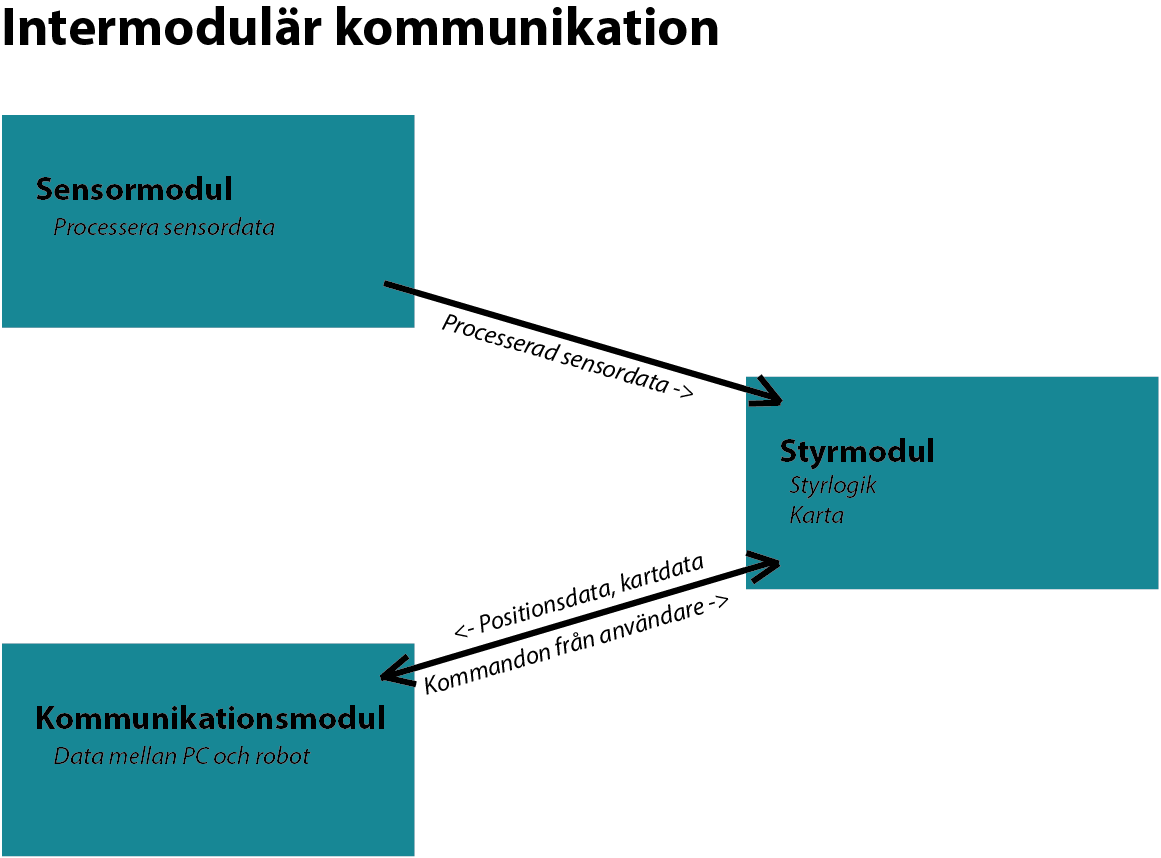
\includegraphics[width=0.5\linewidth]{../Images/Intermodular_Komm}
\caption{Grov skiss av de tre stora modulerna}
\label{fig:Intermodulär_Komm}
\end{figure}



\section{Delsystem 1 - Sensormodul}
Sensormodulens uppgift är att känna av omgivningen runtomkring roboten och behandla denna data för att skicka behandlad data med rätt gränssnitt till styrmodulen.


\subsection{Sensorer}
Sensorerna består främst av IR- och optiska sensorer men även andra typer kan komma att användas. Sensorerna kopplas till mikroprocessorn i sensormodulen som tar hand om all deras data.

Det kommer finnas 6-7 avståndssensorer på roboten, 2 sensorer på höger- och vänster sida, samt framsidan (i färdriktningen). Eventuellt en avståndssensor bak. På vardera sida kommer det sitta Optisk avståndsmätare för kortare avstånd (4-30 cm) och för längre avstånd (10-80 cm). Eventuellt kommer även ultraljudssensorer att användas och optiska avståndsmätare för större avstånd. 

\bigskip

På undersidan kommer en reflexsensor/reflexsensormodul sitta för att detektera start och mål. Denna reflexsensor använder infrarött ljus.$^{[1]}$ 

\bigskip

En vinkelhastighetssensor$ ^{[4]} $ kommer vara placerad på roboten och kopplad till sensormodulen för att avgöra vridning.

\subsection{RFID}
För detektion av RFID-tag kommer en RFID Card Reader, Serial (\#28140) användas. Denna/dessa kommer vara placerad(-e) på sidorna av roboten.

\section{Delsystem 2 - Styrmodul}
Styrmodulen ska kunna ta in data både från sensormodulen och från kommunikationsmodulen beroende på om roboten ligger i autonomt eller manuellt läge. När roboten är i autonomt läge får den strömmande data från sensormodulen som den sedan jämför med kartan som roboten själv bygger upp. Med informationen den fått och har görs ett beslut om vart den ska. När roboten vet vart den ska används reglerteknik för att hålla sig centrerad och att svänga utan att fastna mot väggar.    


\subsection{LCD-Display}
Displayen kommer vara fäst på roboten synligt. Data som skickas till displayen är de beslut som styrmodulen har tagit, status och data från sensorer och kommunikationsmudulen.

\subsection{Motorer}
Motorerna styrs parvis (båda på höger sida och båda på vänster sida) med två signaler per sida. Roboten styrs differentiellt, det vill säga genom olika hastighet på höger och vänster sida. 

\subsection{Gripklo}
Roboten kommer att utrustas med en gripklo för att kunna greppa och släppa material till de nödställda. Gripklon kommer kopplas till strymodulen som ger instruktioner när den ska greppa och släppa. Gripklon kommer att sitta på antingen framsidan eller baksidan av roboten. Upplockning och greppning sker i enlighet med Banspecifikation och tävlingsregler. $^{[2]}$$^{[3]}$

\subsection{Gränssnitt - Display}
Displayen ska visa aktuell status och data från roboten på ett tydligt vis.

\subsection{Brytare för val av autonom eller manuell styrning}
En brytare kommer sitta på ett bra ställe på roboten så den autonoma styrningen kan slås av till fördel av manuell styrning via kommunikationsmodulen och tvärt om med fördel för den autonoma styrningen via sensorer.

\section{Delsystem 3 - Kommunikationsmodul}
Kommunikationsmodulen har två roller beroende på om roboten ligger i autonomt eller manuellt läge. I autonomt läge har den i huvuduppgift att skicka data till PC:n från sensor- och styr-modulen. I manuellt läge har den i uppgift att ta emot data från PC:n som styr roboten via kommunikationsmodulen.

\subsection{Bluetooth - Kommunikationsmodul}
På kommunikationsmodulen sitter det ett Bluetooth-modem som kan skicka och ta emot data från en PC.  

\section{Delsystem 4 - PC}
PC:n har två roller  beroende på om roboten ligger i autonomt eller manuellt läge. I autonomt läge har den i huvuduppgift att ta emot data från roboten och sammanfatta för att rita upp en karta på skärm.

\subsection{Användargränssnitt - Visualisering}
I användargränssnittet så kommer det dels finnas en visualisering av den karta som roboten ritar upp, dels så kommer mät- och styrdata samt de styrbeslut som roboten tar att presenteras på ett tydligt sätt.

\subsection{Bluetooth - PC}
På PC:n sitter det ett Bluetooth-modem som kan skicka och ta emot data från roboten.  


\setcounter{secnumdepth}{0}
\pagebreak
\section{Referenser}


$^{[1]}$Vanheden, ISY:s datablad: \url{https://docs.isy.liu.se/twiki/bin/view/VanHeden} \\[0.1in]

$^{[2]}$Tävlingsregler för TSEA56 2015, Undsättningsrobot: Tävlingsregler0.4.pdf \\[0.1in]

$^{[3]}$Banspecifikation för TSEA56 2015, Undsättningsrobot: Banspec0.3.pdf \\[0.1in]

$^{[4]}$Vanheden, ISY:s datablad, MLX90609: \url{https://docs.isy.liu.se/twiki/pub/VanHeden/DataSheets/MLX90609_datasheet.pdf} \\[0.1in]


\setcounter{secnumdepth}{2}



\end{flushleft}




\end{document}


